\documentclass[12pt]{article}

\usepackage[spanish]{babel}
\usepackage{amsmath, amssymb}
\usepackage{graphicx}
\usepackage{float}
\usepackage{geometry}
\geometry{margin=2.5cm}

\title{Práctica Tema 9: Métodos de relajación para problemas de contorno}
\author{Andrés López Serna}
\date{24 de abril de 2026}

\begin{document}

\maketitle

\begin{abstract}

En esta práctica se estudian métodos de relajación aplicados a problemas de contorno en ecuaciones diferenciales ordinarias y en derivadas parciales. En particular, se analiza el movimiento de una partícula bajo gravedad con condiciones de contorno en el tiempo y el potencial electrostático en un condensador cilíndrico. En ambos casos se implementa el método de Gauss-Seidel para obtener soluciones numéricas estables.

\end{abstract}

\section{Introducción}

Los métodos de relajación constituyen una herramienta fundamental en física computacional para la resolución de problemas de contorno. A diferencia de los métodos de integración directa, que necesitan de condiciones iniciales, estos permiten obtener la solución global de una ecuación diferencial a partir de condiciones impuestas únicamente en los extremos del dominio (condiciones de contorno).

En esta práctica se estudian dos sistemas físicos distintos. Por un lado, se estudia el movimiento de una partícula sometida a aceleración constante bajo condiciones de contorno en el tiempo, donde se resuelve la ecuación diferencial que gobierna su dinámica. Por otro lado, se analiza el potencial electrostático en un condensador cilíndrico, donde se resuelve la ecuación de Laplace en coordenadas cilíndricas mediante discretización espacial. En ambos problemas desconocemos las condiciones iniciales completas (en la dinámica falta la velocidad inicial y en el cilindro nos falta el potencial en su interior), pero conocemos sus condiciones de contorno, lo que justifica el uso de métodos iterativos de relajación.

\section{Marco teórico}

\subsection{Método de Gauss-Seidel}

El método de Gauss-Seidel consiste en resolver sistemas discretizados de ecuaciones diferenciales mediante iteración sucesiva, actualizando cada punto del dominio con los valores más recientes disponibles. El criterio de convergencia se basa en la variación máxima entre iteraciones:

\begin{equation}
\delta = \max_i |x_i^{(n+1)} - x_i^{(n)}|
\end{equation}

El proceso se detiene cuando $\delta < \varepsilon$, donde $\varepsilon$ es la tolerancia, garantizando estabilidad numérica.

\subsection{Discretización de la segunda derivada}

Para el problema dinámico se utiliza la aproximación de diferencias centradas que en el problema de la bola es:

\begin{equation}
\frac{x_{i-1} - 2x_i + x_{i+1}}{h^2} = -g
\end{equation}

despejando se puede obtener la siguiente relación iterativa:

\begin{equation}
x_i = \frac{1}{2}\left(x_{i-1} + x_{i+1} + g h^2 \right)
\label{iter_A}
\end{equation}

\subsection{Ecuación de Laplace en coordenadas cilíndricas}

El potencial electrostático en coordenadas cilíndricas satisface:

\begin{equation}
\frac{1}{r}\frac{d}{dr}\left(r \frac{dV}{dr}\right) = 0
\end{equation}

lo que se puede reescribir de forma que se pueda resolver directamente mediante diferencias finitas:

\begin{equation}
\frac{d^2 V}{dr^2} + \frac{1}{r}\frac{dV}{dr} = 0
\label{laplace}
\end{equation}

\section{OPCIÓN A: Movimiento de una bola}

\subsection{Planteamiento físico}

Se estudia el movimiento de una partícula bajo aceleración gravitatoria constante:

\begin{equation}
\frac{d^2 x}{dt^2} = -g
\end{equation}

con condiciones de contorno:

\begin{equation}
x(0)=0, \quad x(10)=0
\end{equation}

Se trata de un problema de contorno donde la velocidad inicial no es conocida a priori, al menos, no es necesario conocerla ya que se puede resolver el problema utilizando la relación iterativa de la ecuación \ref{iter_A}.

No obstante, la expresión analítica que gobierna el movimiento parabólico es $x(t) = v_0\cdot t - \frac{1}{2} g t^2$. Imponiendo en esta ecuación que $x(10)=0$ se llega a que $v_0=\frac{1}{2}g\cdot10\approx 49.05\text{ } m/s$.

\subsection{Resultados}

La Figura~\ref{fig:bola} muestra la comparación entre la solución numérica y la solución analítica.

\begin{figure}[H]
\centering

\begin{minipage}{0.48\textwidth}
    \centering
    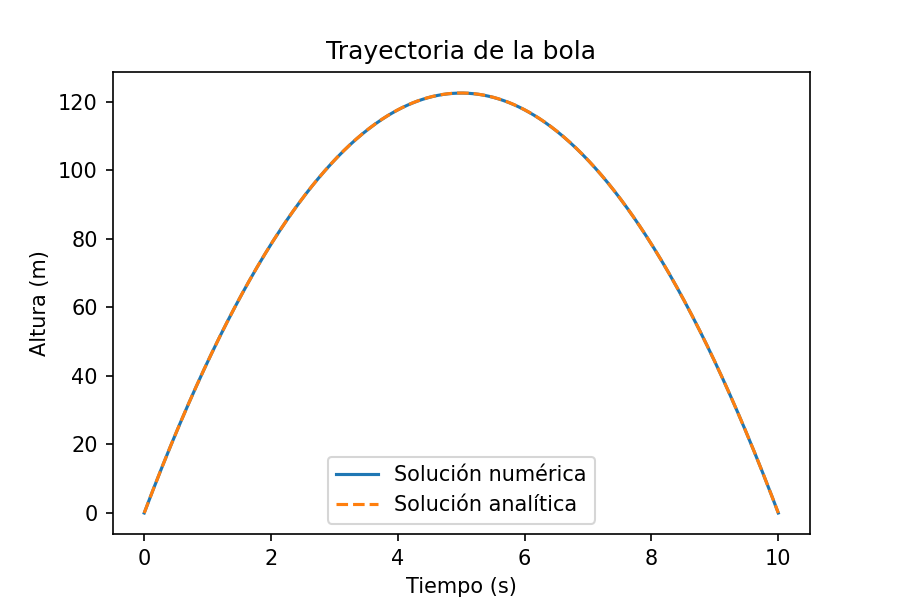
\includegraphics[width=\textwidth]{imagenes/trayectoria_bola_A.png}
    \caption{Trayectoria de la bola obtenida mediante Gauss-Seidel comparada con la solución analítica.}
    \label{fig:bola}
\end{minipage}
\hfill
\begin{minipage}{0.48\textwidth}
    \centering
    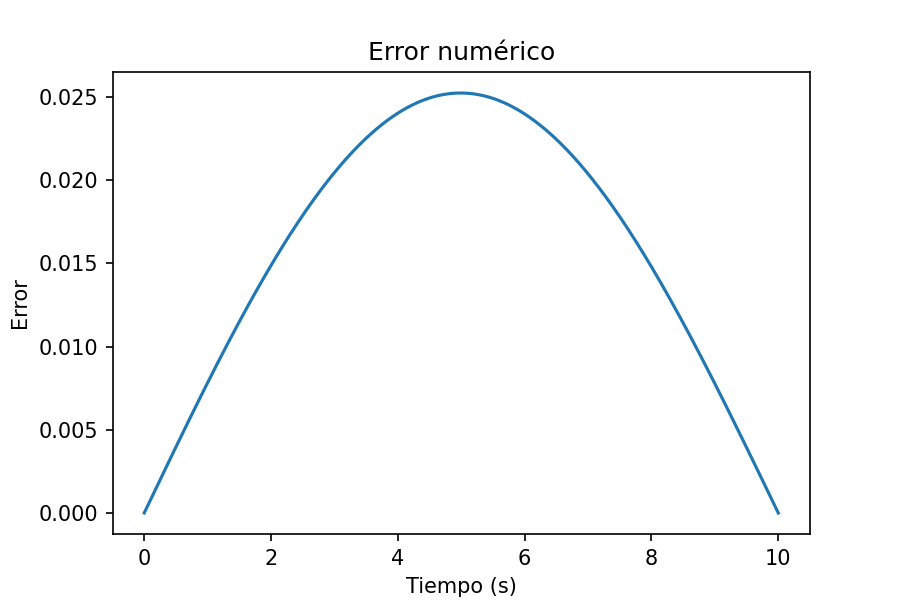
\includegraphics[width=\textwidth]{imagenes/errorA_2D.png}
    \caption{Error absoluto entre solución numérica y analítica.}
    \label{fig:errorA}
\end{minipage}

\end{figure}

Se observa una excelente concordancia entre ambas soluciones, reproduciendo la trayectoria parabólica esperada. Además, en la figura ~\ref{fig:errorA} se muestra el error numérico permanece despreciable durante todo el dominio.

Finalmente, como conocemos la velocidad inicial, podemos obtenerla también aproximadamente sencillamente utilizando que $v_0\approx \frac{x_1-x_0}{t_1-t_0}\approx 48.94$ lo cual resulta en un margen de error inferior al 0.5\% respecto al valor analítico.

\section{OPCIÓN B: Condensador cilíndrico (1D)}

\subsection{Planteamiento físico}

En la opción B se estudia un condensador cilíndrico con su radio interior $R_i=1\,cm$ mantenido a un potencial $V(R_i)=2.5\,V$ y su radio exterior $R_e=4\,cm$ a un potencial $V(R_e)=0$.

Las simetrías propias del problema permiten reducirlo a únicamente la dimensión radial. La solución analítica de la ecuación de Laplace en este caso es la siguiente:

\begin{equation}
V(r) = V_i \frac{\ln(R_e/r)}{\ln(R_e/R_i)}
\end{equation}

Por otro lado, la resolución de la ecuación de Laplace (ecuación \ref{laplace}) de forma numérica lleva a una discretización que introduce un factor geométrico ($\alpha_i = \frac{h}{2r_i}$) que modifica los pesos de los nodos vecinos. La relación iterativa obtenida mediante diferencias finitas centradas es la siguiente:

\begin{equation}
V_i^{(n+1)} =
\frac{1}{2}\left[
(1+\alpha_i)V_{i+1}^{(n)} + (1-\alpha_i)V_{i-1}^{(n+1)}
\right]
\end{equation}

\subsection{Resultados numéricos}

La Figura~\ref{fig:Vr} muestra la comparación entre solución numérica y analítica.

\begin{figure}[H]
\centering
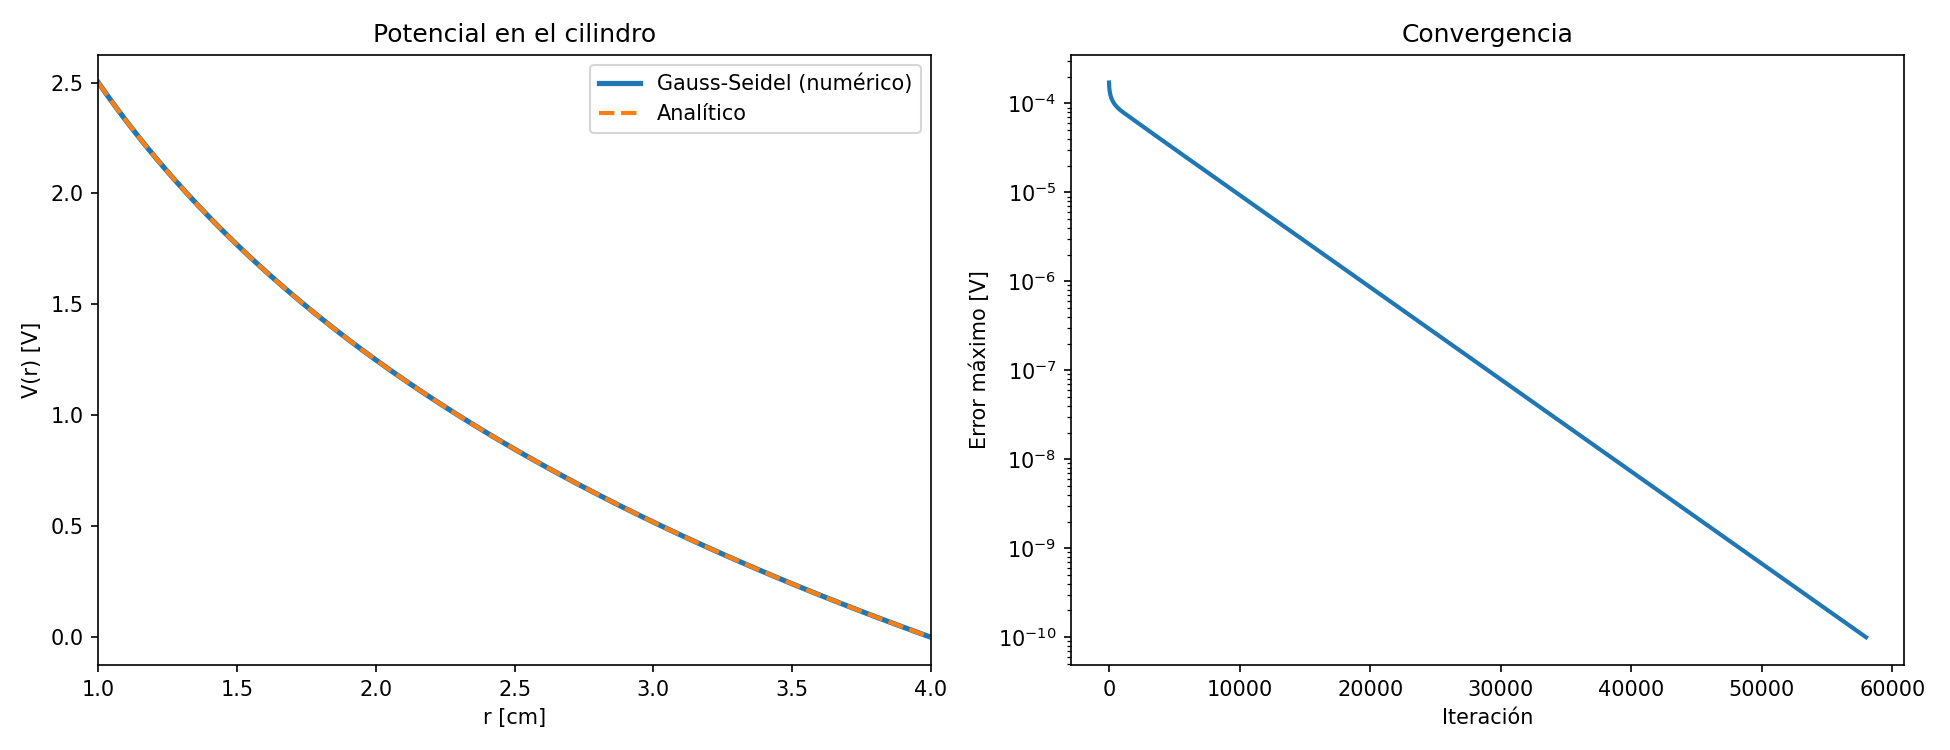
\includegraphics[width=0.75\textwidth]{imagenes/V_r_convergencia.png}
\caption{Potencial radial V(r) y evolución de la convergencia del método.}
\label{fig:Vr}
\end{figure}

Se observa una excelente concordancia con la solución analítica y cómo el potencial decrece con el radio (de forma logarítmica) ya que el potencial del radio interno es mayor que el radio externo. Adicionalmente, se puede observar que al aumentar el número de iteraciones el método se vuelve más preciso, lo cual es propio de un método estable. Finalmente, en la Figura~\ref{fig:mapa1D} se muestra la reconstrucción 2D por simetría axial.

\begin{figure}[H]
\centering
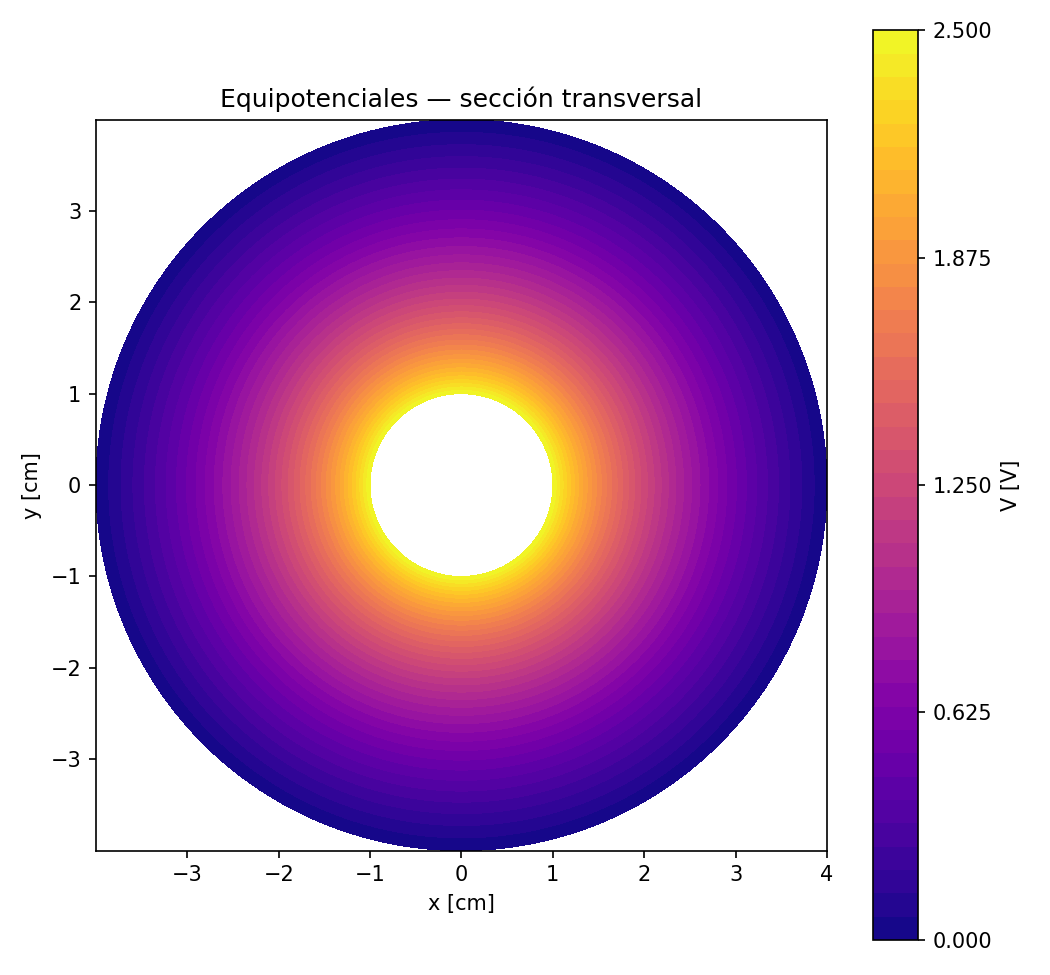
\includegraphics[width=0.62\textwidth]{imagenes/equipotenciales_2D.png}
\caption{Distribución equipotencial en el plano transversal del condensador.}
\label{fig:mapa1D}
\end{figure}

\section{OPCIÓN B variante: dependencia con z}

\subsection{Planteamiento}

Se introduce ahora un condensador cilíndrico de longitud finita $L=20\,cm$, con tapas conectadas a tierra (anteriormente la longitud era la misma pero al no considerar el potencial en las tapas consideramos que podía tomar cualquier valor). El potencial depende ahora de dos variables, $V = V(r,z)$, y satisface:

\begin{equation}
\frac{1}{r}\frac{\partial}{\partial r}\left(r \frac{\partial V}{\partial r}\right)
+
\frac{\partial^2 V}{\partial z^2}
= 0
\end{equation}

Por ello la discretización en una malla $(r,z)$ conduce a la combinación de un término radial y un término axial (más información en Anexo B).

El término radial se aproxima como:



\begin{equation}
V_{rr} =
\frac{1}{2}\left[(1-\alpha_i)V_{i-1,j} + (1+\alpha_i)V_{i+1,j}\right] \text{ donde
$\alpha_i = \frac{dr}{2r_i}$}
\end{equation}

El término axial se discretiza mediante:

\begin{equation}
V_{zz} = \frac{1}{2}\left(V_{i,j+1} + V_{i,j-1}\right)
\end{equation}

La actualización final del esquema de Gauss-Seidel es:

\begin{equation}
V_{i,j}^{(n+1)} = \frac{1}{2}\left(V_{rr} + V_{zz}\right)
\end{equation}

Esta expresión combina la contribución radial (con corrección geométrica cilíndrica) y la contribución axial, permitiendo resolver el problema completo en dos dimensiones y manteniendo la independencia con el ángulo polar.

\subsection{Resultados}

La Figura~\ref{fig:2D_tierra} muestra la distribución del potencial en el plano $(r,z)$.

\begin{figure}[H]
\centering
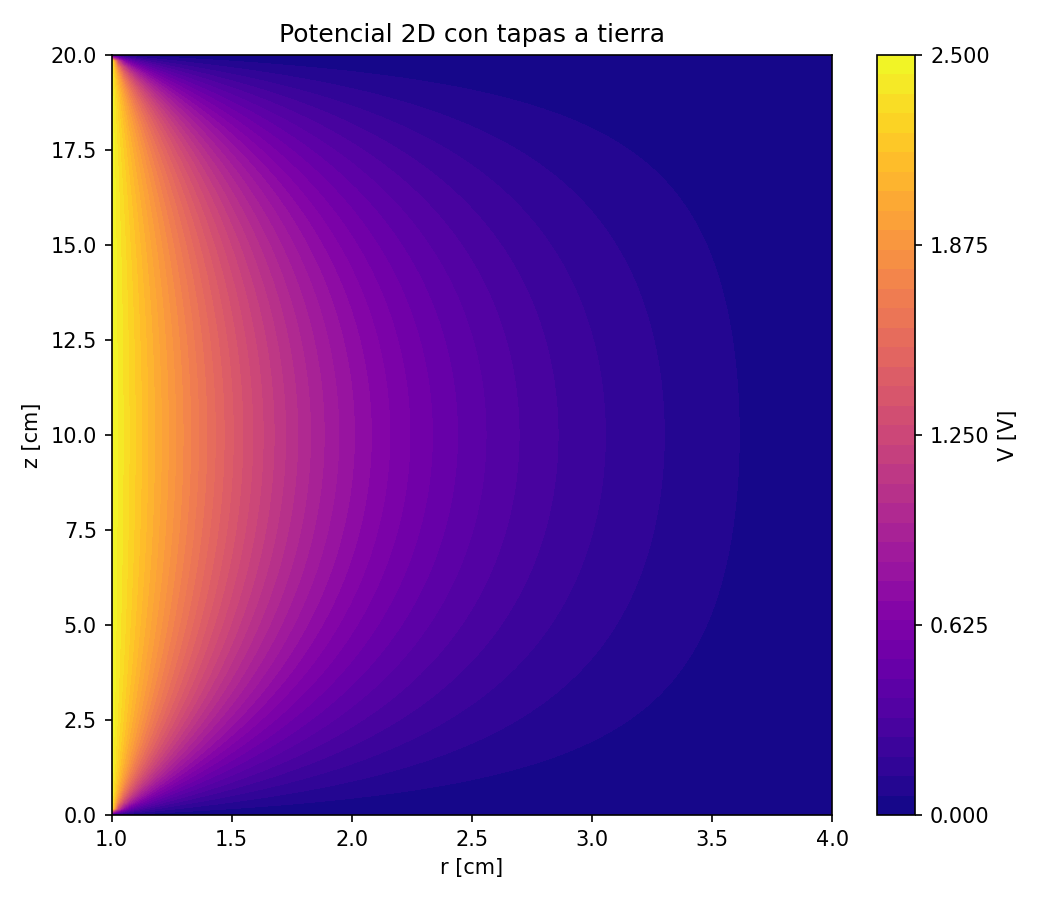
\includegraphics[width=0.75\textwidth]{imagenes/equipotenciales_2D_tierra.png}
\caption{Distribución del potencial en el condensador con tapas a tierra.}
\label{fig:2D_tierra}
\end{figure}

Se observa claramente que el potencial ya no depende únicamente de $r$, sino que presenta variación axial debido a las condiciones de contorno en las tapas. Este efecto es especialmente notorio en las regiones próximas a $z=0$ y $z=L$. La figura \ref{fig:2D_tierra} es un corte del cilindro, pero como el problema posee simetría de revolución, nos da la información completa del problema.

\section{Conclusiones}

Durante la resolución de ambos problemas el método de Gauss-Seidel se ha mostrado eficaz tanto para ecuaciones diferenciales ordinarias como para ecuaciones en derivadas parciales.

En el problema dinámico, permite reconstruir la trayectoria completa sin necesidad de conocer la velocidad inicial (aunque en este caso fuera posible y sencilla de hallar) mientras que en el problema electrostático, se reproduce con gran precisión la solución analítica en el caso unidimensional.

Finalmente, la extensión a dos dimensiones muestra cómo la introducción de condiciones de contorno adicionales rompe la simetría radial e introduce dependencia con la coordenada axial. En conjunto, la práctica ilustra la precisión y rapidez de los métodos de relajación para resolver problemas físicos con condiciones de contorno.


\newpage
\appendix
\section*{Anexo A: Variables y parámetros del modelo}

En este anexo se recogen las variables y parámetros utilizados a lo largo de la práctica y el informe.

\begin{center}
\begin{tabular}{ll}
\hline
\textbf{Variable} & \textbf{Significado} \\
\hline

$x(t)$ & Posición de la partícula en función del tiempo (problema A) \\

$t$ & Tiempo en segundos, variable independiente del problema dinámico \\

$g$ & Aceleración de la gravedad ($9.81\,m/s^2$), fuerza constante aplicada \\

$h$ & Paso de discretización temporal en la malla $t_i$ \\

$N$ & Número de puntos de la malla temporal en el problema A \\

$\varepsilon$ & Criterio de convergencia del método de Gauss-Seidel \\

$\delta$ & Error máximo entre iteraciones sucesivas \\

$x_i$ & Aproximación numérica de la posición en el nodo temporal $i$ \\

$v_0$ & Velocidad inicial de la partícula (no conocida a priori) \\

$x_{\text{exact}}$ & Solución analítica de la ecuación de movimiento \\

\\
\hline
$V(r)$ & Potencial electrostático en función de la coordenada radial \\

$r$ & Coordenada radial en el condensador cilíndrico \\

$R_i$ & Radio del cilindro interior \\

$R_e$ & Radio del cilindro exterior \\

$L$ & Longitud del condensador cilíndrico \\

$V_i$ & Potencial del cilindro interior \\

$V_e$ & Potencial del cilindro exterior (tierra) \\

$V_{i,j}$ & Potencial numérico en la malla 2D (problema con dependencia en $z$) \\

$dr$ & Paso de discretización radial \\

$dz$ & Paso de discretización axial \\

\\
\hline
$V(r,z)$ & Potencial electrostático en el caso bidimensional \\

$z$ & Coordenada axial del condensador cilíndrico \\

$Nr$ & Número de puntos en la dirección radial \\

$Nz$ & Número de puntos en la dirección axial \\

$\alpha$ & Factor geométrico cilíndrico $\alpha = \frac{dr}{2r}$ \\

$V_{rr}$ & Aproximación discreta del término radial de Laplace \\

$V_{zz}$ & Aproximación discreta del término axial de Laplace \\

\\
\hline
$\Delta V$ & Variación del potencial entre iteraciones \\

$\nabla^2 V$ & Operador Laplaciano en coordenadas cilíndricas \\

$\text{it}$ & Número de iteraciones del método de relajación \\

$\text{max\_iter}$ & Número máximo de iteraciones permitidas \\

\hline
\end{tabular}
\end{center}

\newpage
\section*{Anexo B: Derivación de las relaciones iterativas}

En este anexo se deriva de forma explícita la obtención de las ecuaciones iterativas empleadas en los métodos de relajación (Gauss-Seidel) para los dos problemas estudiados en la práctica.

\subsection*{B.1 Problema A: ecuación de movimiento en 1D}

La ecuación diferencial del movimiento bajo gravedad es:

\begin{equation}
\frac{d^2 x}{dt^2} = -g
\end{equation}

Se discretiza el dominio temporal en una malla uniforme $t_i = t_0 + i h$, donde $h$ es el paso temporal.

La segunda derivada se aproxima mediante diferencias centradas:

\begin{equation}
\frac{d^2 x}{dt^2} \approx \frac{x_{i-1} - 2x_i + x_{i+1}}{h^2}
\end{equation}

Sustituyendo en la ecuación diferencial:

\begin{equation}
\frac{x_{i-1} - 2x_i + x_{i+1}}{h^2} = -g
\end{equation}


Finalmente, despejando $x_i$ se obtiene la relación iterativa:

\begin{equation}
x_i = \frac{1}{2}\left(x_{i-1} + x_{i+1} + g h^2 \right)
\end{equation}

\subsection*{B.2 Problema B: ecuación de Laplace en coordenadas cilíndricas (1D radial)}

La ecuación de Laplace en coordenadas cilíndricas con simetría axial es:

\begin{equation}
\frac{1}{r}\frac{d}{dr}\left(r \frac{dV}{dr}\right) = 0
\end{equation}

Se expande el operador:

\begin{equation}
\frac{d^2 V}{dr^2} + \frac{1}{r}\frac{dV}{dr} = 0
\end{equation}

Se discretiza el dominio radial con paso $h$:

\begin{equation}
\frac{d^2 V}{dr^2} \approx \frac{V_{i+1} - 2V_i + V_{i-1}}{h^2}
\text{;     }
\frac{dV}{dr} \approx \frac{V_{i+1} - V_{i-1}}{2h}
\end{equation}

Sustituyendo:

\begin{equation}
\frac{V_{i+1} - 2V_i + V_{i-1}}{h^2}
+
\frac{1}{r_i}\frac{V_{i+1} - V_{i-1}}{2h}
= 0
\end{equation}

Multiplicando por $h^2$:

\begin{equation}
V_{i+1} - 2V_i + V_{i-1}
+
\frac{h}{2r_i}(V_{i+1} - V_{i-1}) = 0
\end{equation}

Definiendo $\alpha_i = \frac{h}{2r_i}$ se obtiene:

\begin{equation}
(1+\alpha_i)V_{i+1} + (1-\alpha_i)V_{i-1} - 2V_i = 0
\end{equation}

Despejando $V_i$:

\begin{equation}
V_i =
\frac{1}{2}\left[
(1+\alpha_i)V_{i+1} + (1-\alpha_i)V_{i-1}
\right]
\end{equation}

\subsection*{B.3 Problema B extendido: ecuación 2D $(r,z)$}

En el caso con dependencia en $z$, la ecuación de Laplace es:

\begin{equation}
\frac{1}{r}\frac{\partial}{\partial r}\left(r \frac{\partial V}{\partial r}\right)
+
\frac{\partial^2 V}{\partial z^2}
= \frac{\partial^2 V}{\partial r^2} + \frac{1}{r}\frac{\partial V}{\partial r}
+
\frac{\partial^2 V}{\partial z^2}
= 0
\end{equation}

Se discretizan las derivadas:

\begin{equation}
\frac{\partial^2 V}{\partial r^2}
\approx
\frac{V_{i+1,j} - 2V_{i,j} + V_{i-1,j}}{dr^2}; \frac{\partial V}{\partial r}
\approx
\frac{V_{i+1,j} - V_{i-1,j}}{2dr};\frac{\partial^2 V}{\partial z^2}
\approx
\frac{V_{i,j+1} - 2V_{i,j} + V_{i,j-1}}{dz^2}
\end{equation}

Sustituyendo en la ecuación de Laplace:

\begin{equation}
\frac{V_{i+1,j} - 2V_{i,j} + V_{i-1,j}}{dr^2}
+
\frac{1}{r_i}\frac{V_{i+1,j} - V_{i-1,j}}{2dr}
+
\frac{V_{i,j+1} - 2V_{i,j} + V_{i,j-1}}{dz^2}
= 0
\end{equation}

Definiendo ahora $\alpha_i = \frac{dr}{2r_i}$, para el término radial llegamos a:

\begin{equation}
V_{rr} =
\frac{1}{2}\left[
(1+\alpha_i)V_{i+1,j} + (1-\alpha_i)V_{i-1,j}
\right]
\end{equation}

Por otro lado, obtenemos el siguiente término axial:

\begin{equation}
V_{zz} =
\frac{1}{2}\left(V_{i,j+1} + V_{i,j-1}\right)
\end{equation}

Finalmente, la relación iterativa queda:

\begin{equation}
V_{i,j}^{(n+1)} =
\frac{1}{2}\left(V_{rr} + V_{zz}\right)
\end{equation}
\end{document}
